\appendix
\chapter{Allegati}
\label{appendix:SWMM}
\section{Tabelle e immagini da SWMM}
%
\begin{figure}[H]
    \centering
    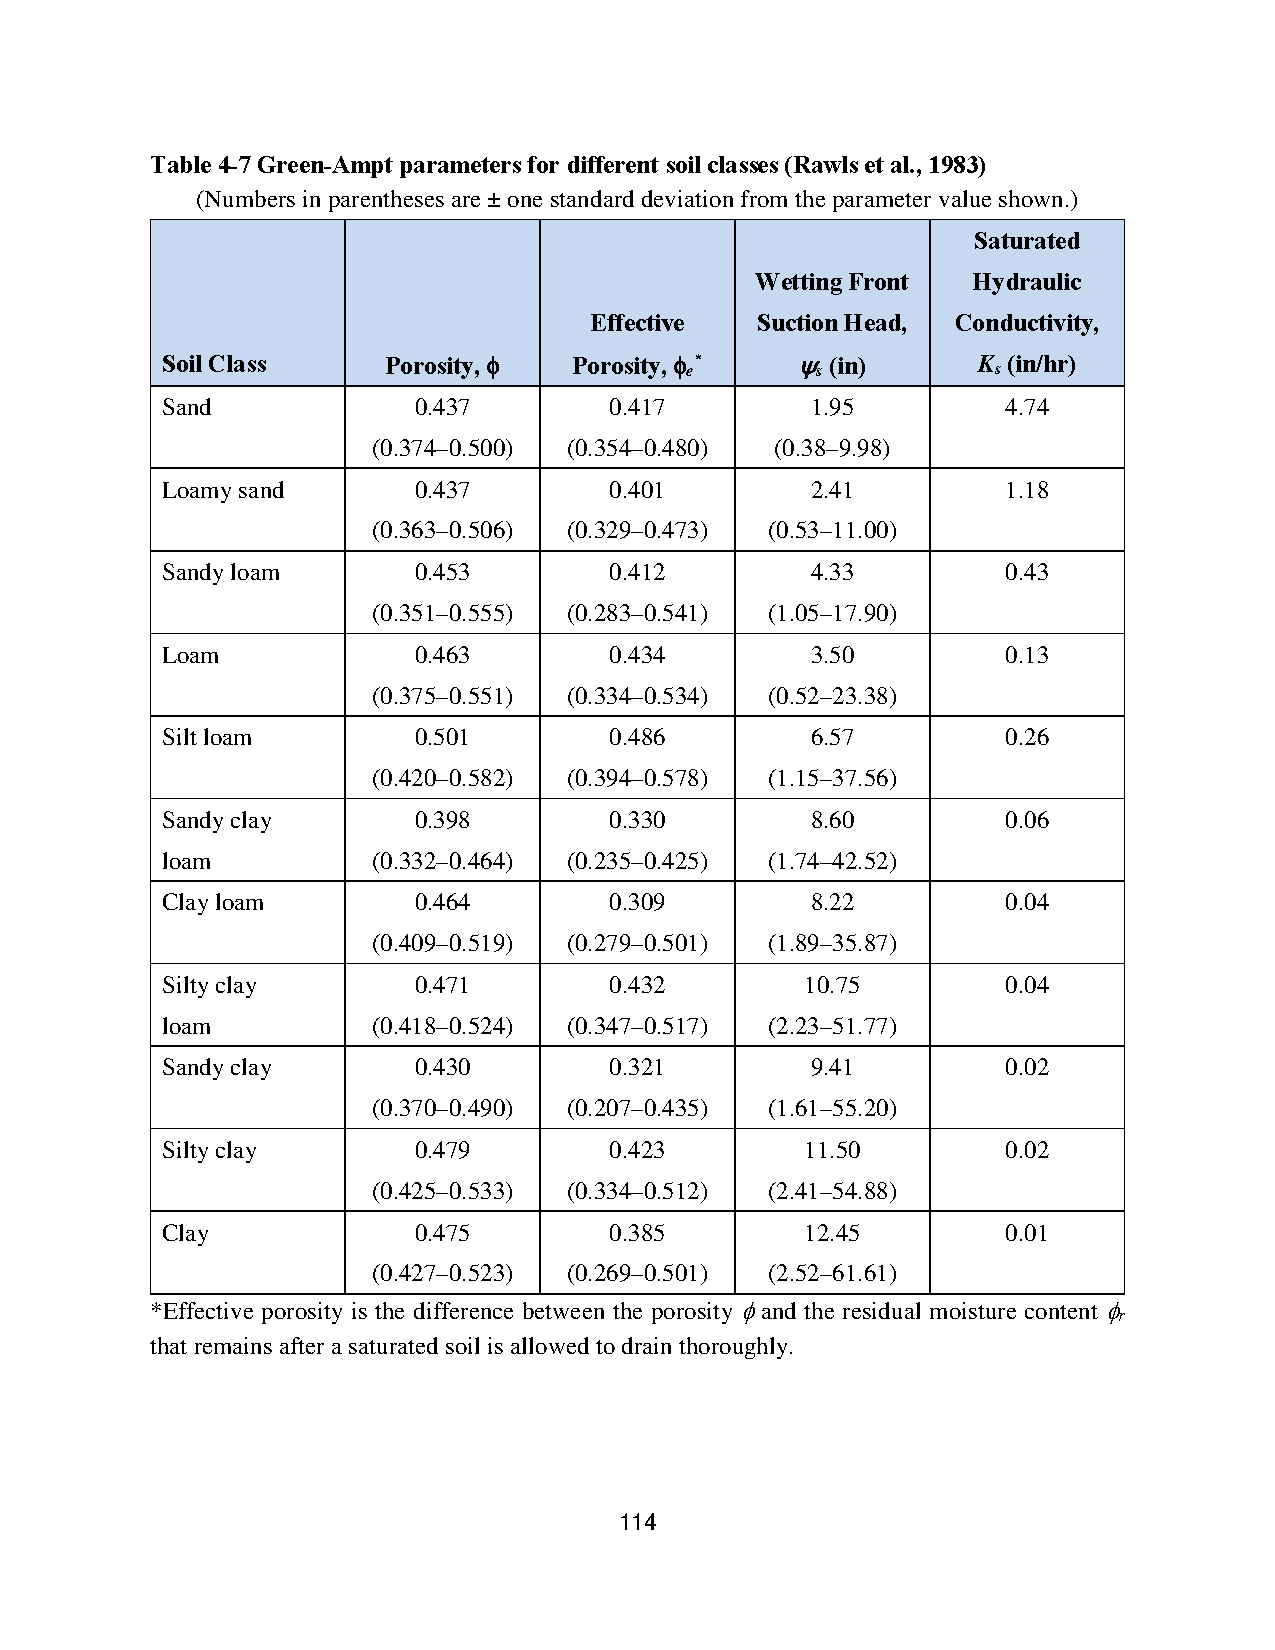
\includegraphics[trim=2.5cm 4.5cm 2.5cm 3.6cm,clip,width=\textwidth]{IMG/table4-7_Ks.pdf} 
    \caption[Tabella 4.7 di SWMM]{Tabella 4.7 di SWMM Green-Ampt parameters for different soil classes (Rawls et al., 1983) (Numbers in parentheses are ± one standard deviation from the parameter value shown.)}
    \label{SWMM:tabella4-7}
\end{figure}

%\chapter{Rete di smaltimento delle acque meteoriche allo stato di progetto (con presenza della rete di drenaggio) - tutti i mancanti}
%\label{appendix:FasiIntermedie}
%\section{Progetto sbagliato}
%\section{Progetto con solo i LID}
%\TabellaDiametriCondotte{Diametri progetti conduct-mod LID. In verde sono indicati i valori che hanno subito una modifica rispetto al progetto senza LID}{tab:Diametri_conduct-mod-LID}{IMG/Diametri-conduct-mod-LID.tex}
%\TabellaVerificheLinkFLow{Progetto con aggiunta dei soli LID -- Verifiche di massima velocità, riempimento condotta e del criterio di autopulizia}{tab:LinkFlow_Verifiche-MOD-LID}{IMG/LinkFlow-Verifiche-MOD-LID.tex}
%\section{Progetto con vasche e lid rifatto dopo i lid}
%\section{Progetto con vasche e lid sistemato}
%
\section{Codici di input SWMM per i LID e relative immagini}
\begin{landscape}
\begin{figure}[H]
    \centering
    % \subfloat[][\emph{Campata 1\label{fig:MomentiUnitariA}}]
    \subfloat[][\emph{Parametri del sottobacino}]{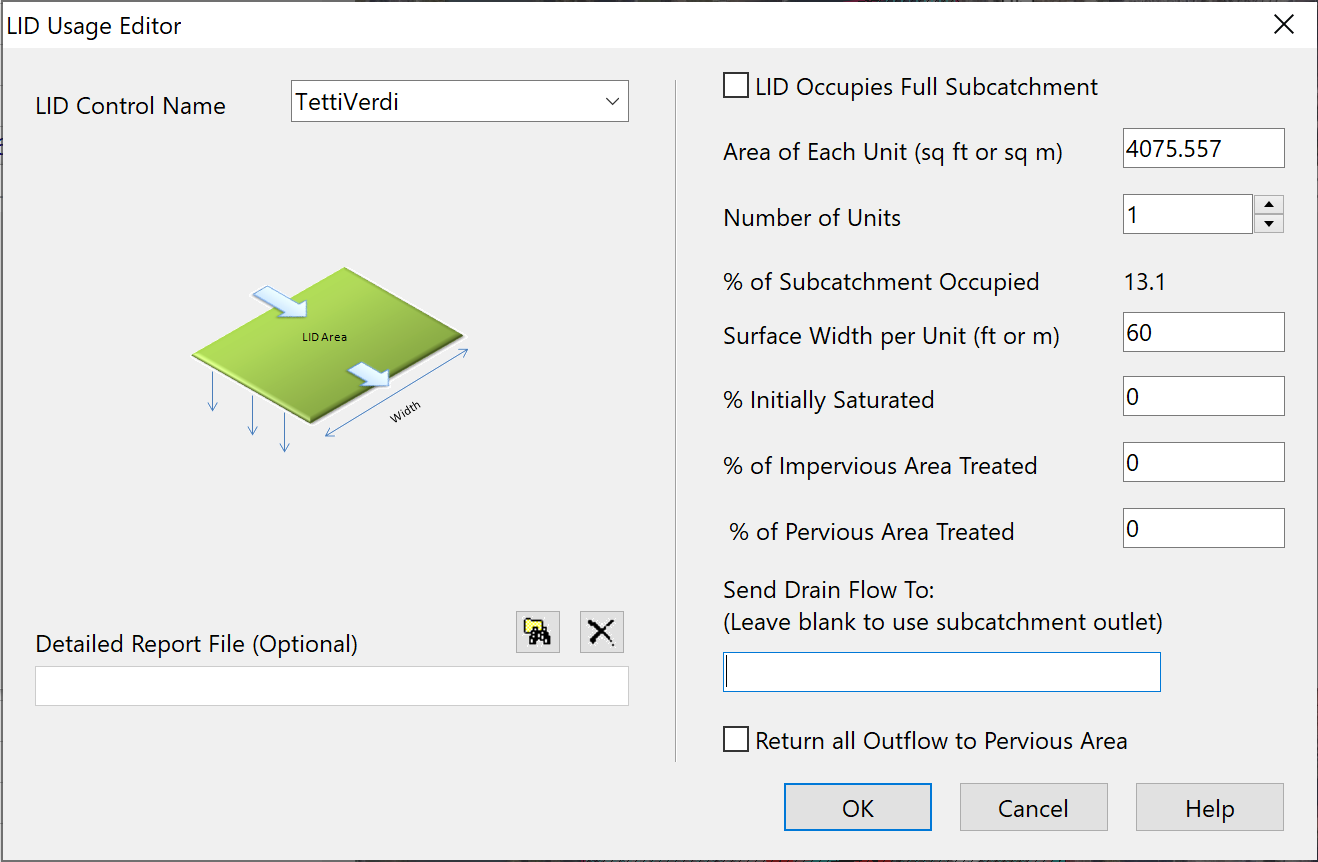
\includegraphics[height=0.45\textheight]{IMG/LID-Inflow/LID0.png}} 
    \subfloat[][\emph{Tetto verde}]{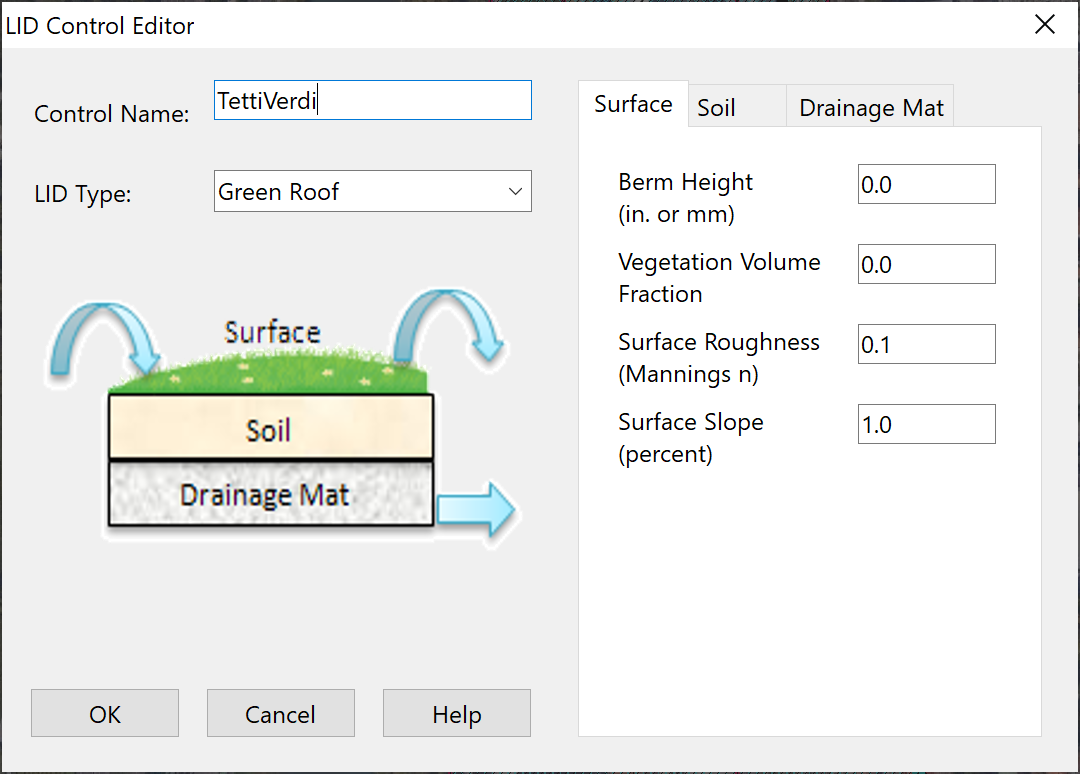
\includegraphics[height=0.45\textheight]{IMG/LID-Inflow/LID1.png}} \\
    \subfloat[][\emph{Pavimento permeabile}]{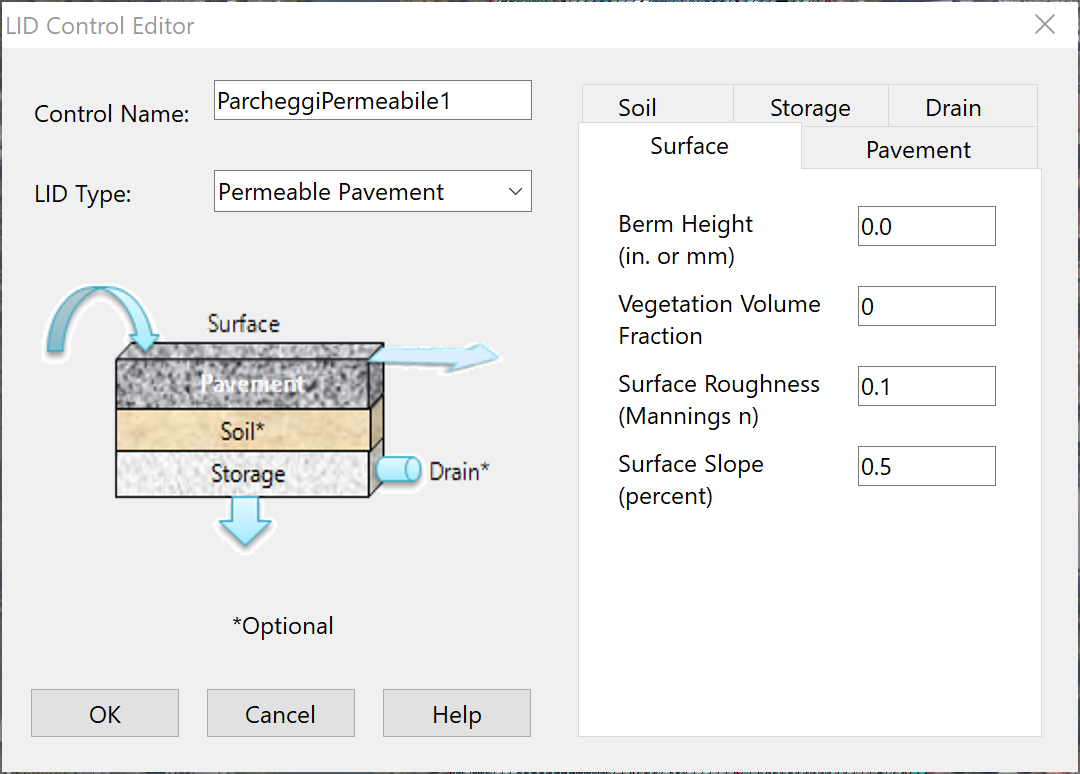
\includegraphics[height=0.45\textheight]{IMG/LID-Inflow/LID2.png}}
    \subfloat[][\emph{Celle di bio-ritenzione}]{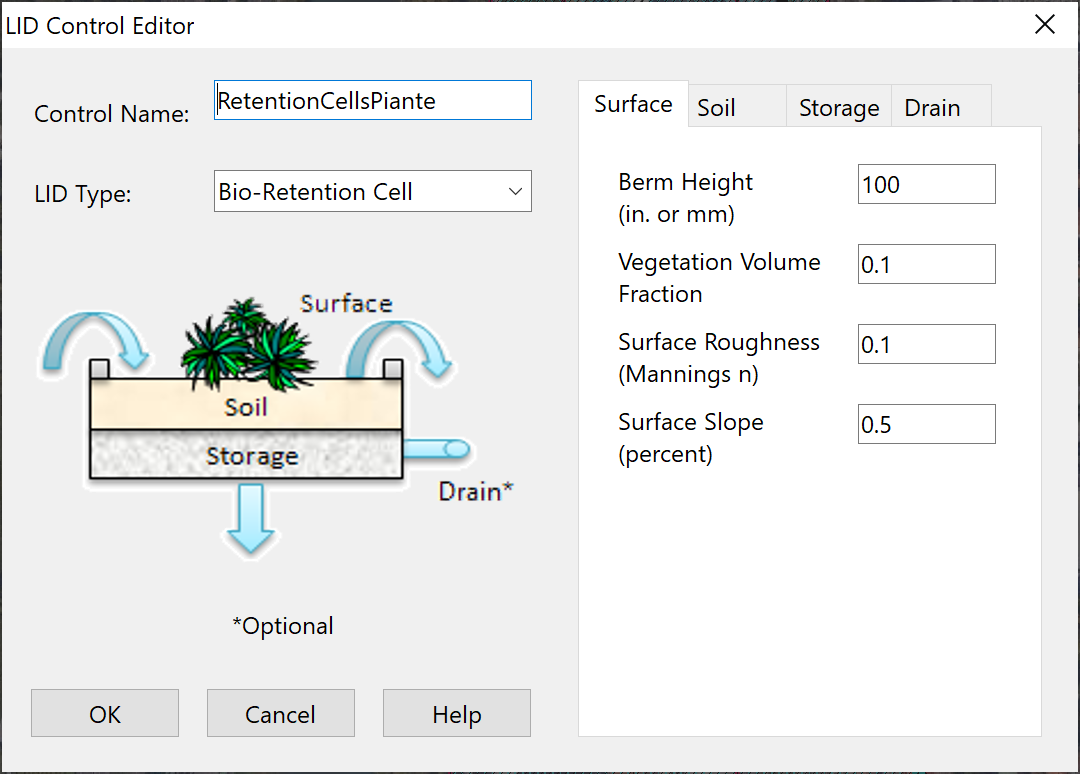
\includegraphics[height=0.45\textheight]{IMG/LID-Inflow/LID3.png}}\\
\caption{Schermate SWMM riguardo i parametri dei LID}
%\label{fig:ProfiliProgettoCondotte}
\end{figure}
\end{landscape}
\begin{lstlisting}
    [LID_CONTROLS]
    ;;Name               Type/Layer Parameters
    ;;--------------     ---------- ----------
    ParcheggiPermeabile1 PP
    ParcheggiPermeabile1 SURFACE    0.0        0     0.1   0.5  5
    ParcheggiPermeabile1 PAVEMENT   150        0.15  0.4   360  0     0    0
    ParcheggiPermeabile1 STORAGE    300        0.3   0.5   0
    ParcheggiPermeabile1 DRAIN      0          0.5   6     6    0     0
    TettiVerdi           GR
    TettiVerdi           SURFACE    0.0        0.0   0.1   1.0  5
    TettiVerdi           SOIL       100        0.5   0.4   0.1  2000  40   70
    TettiVerdi           DRAINMAT   50         0.3   0.01
    RetentionCellsPiante BC
    RetentionCellsPiante SURFACE    100        0.1   0.1   0.5  5
    RetentionCellsPiante SOIL       300        0.5   0.2   0.1  4     35   3.5
    RetentionCellsPiante STORAGE    200        0.75  0.5   0
    RetentionCellsPiante DRAIN      0          0.5   6     6    0     0
    \end{lstlisting}
    \begin{landscape}
    \begin{lstlisting}[basicstyle=\scriptsize\ttfamily,numberstyle=\tiny]
    [LID_USAGE]
    ;;Subcatchment   LID                  Process Number     Area    Width  InitSat  FromImp  ToPerv  RptFile  DrainTo  FromPerv
    ;;-------------- ----------------     ------- ---------  ------  -----  -------  -------  ------  -------- --------
    S_2              TettiVerdi           1       1148.864   24.010  0      0        0        *       *        0
    S_2              RetentionCellsPiante 1       1233.037   32      0      0        0        *       *        0
    S_3              TettiVerdi           1       160.533    6.981   0      0        0        *       *        0
    S_4              RetentionCellsPiante 1       337.869    69.486  0      0        0        *       *        0
    S_5              RetentionCellsPiante 1       147.403    36.546  0      0        0        *       *        0
    S_6              TettiVerdi           1       574.006    30.530  0      0        0        *       *        0
    S_6              RetentionCellsPiante 1       401.041    82.5    0      0        0        *       *        0
    S_7              TettiVerdi           1       409.026    32.451  0      0        0        *       *        0
    S_7              RetentionCellsPiante 1       100.528    87.646  0      0        0        *       *        0
    S_10             TettiVerdi           1       441.657    11.003  0      0        0        *       *        0
    S_10             RetentionCellsPiante 1       42.96      52.54   0      0        0        *       *        0
    S_11             TettiVerdi           1       616.205    39.484  0      0        0        *       *        0
    S_11             RetentionCellsPiante 1       97.675     52.54   0      0        0        *       *        0
    S_15             TettiVerdi           1       669.122    37.466  0      0        0        *       *        0
    S_15             RetentionCellsPiante 1       272.261    109.044 0      0        0        *       *        0
    S_18             TettiVerdi           1       709.912    47.5    0      0        0        *       *        0
    S_20             TettiVerdi           1       900.278    36      0      0        0        *       *        0
    S_21             TettiVerdi           1       74.188     12      0      0        0        *       *        0
    S_22             ParcheggiPermeabile1 1       4075.557   60      0      0        0        *       *        0
    S_22             TettiVerdi           1       3911.637   23.4    0      0        0        *       *        0
    S_24             ParcheggiPermeabile1 1       7847.3     130     0      0        0        *       *        0
    \end{lstlisting}
    \end{landscape}
    
%\section{prova}
%\chapter{Computo metrico}
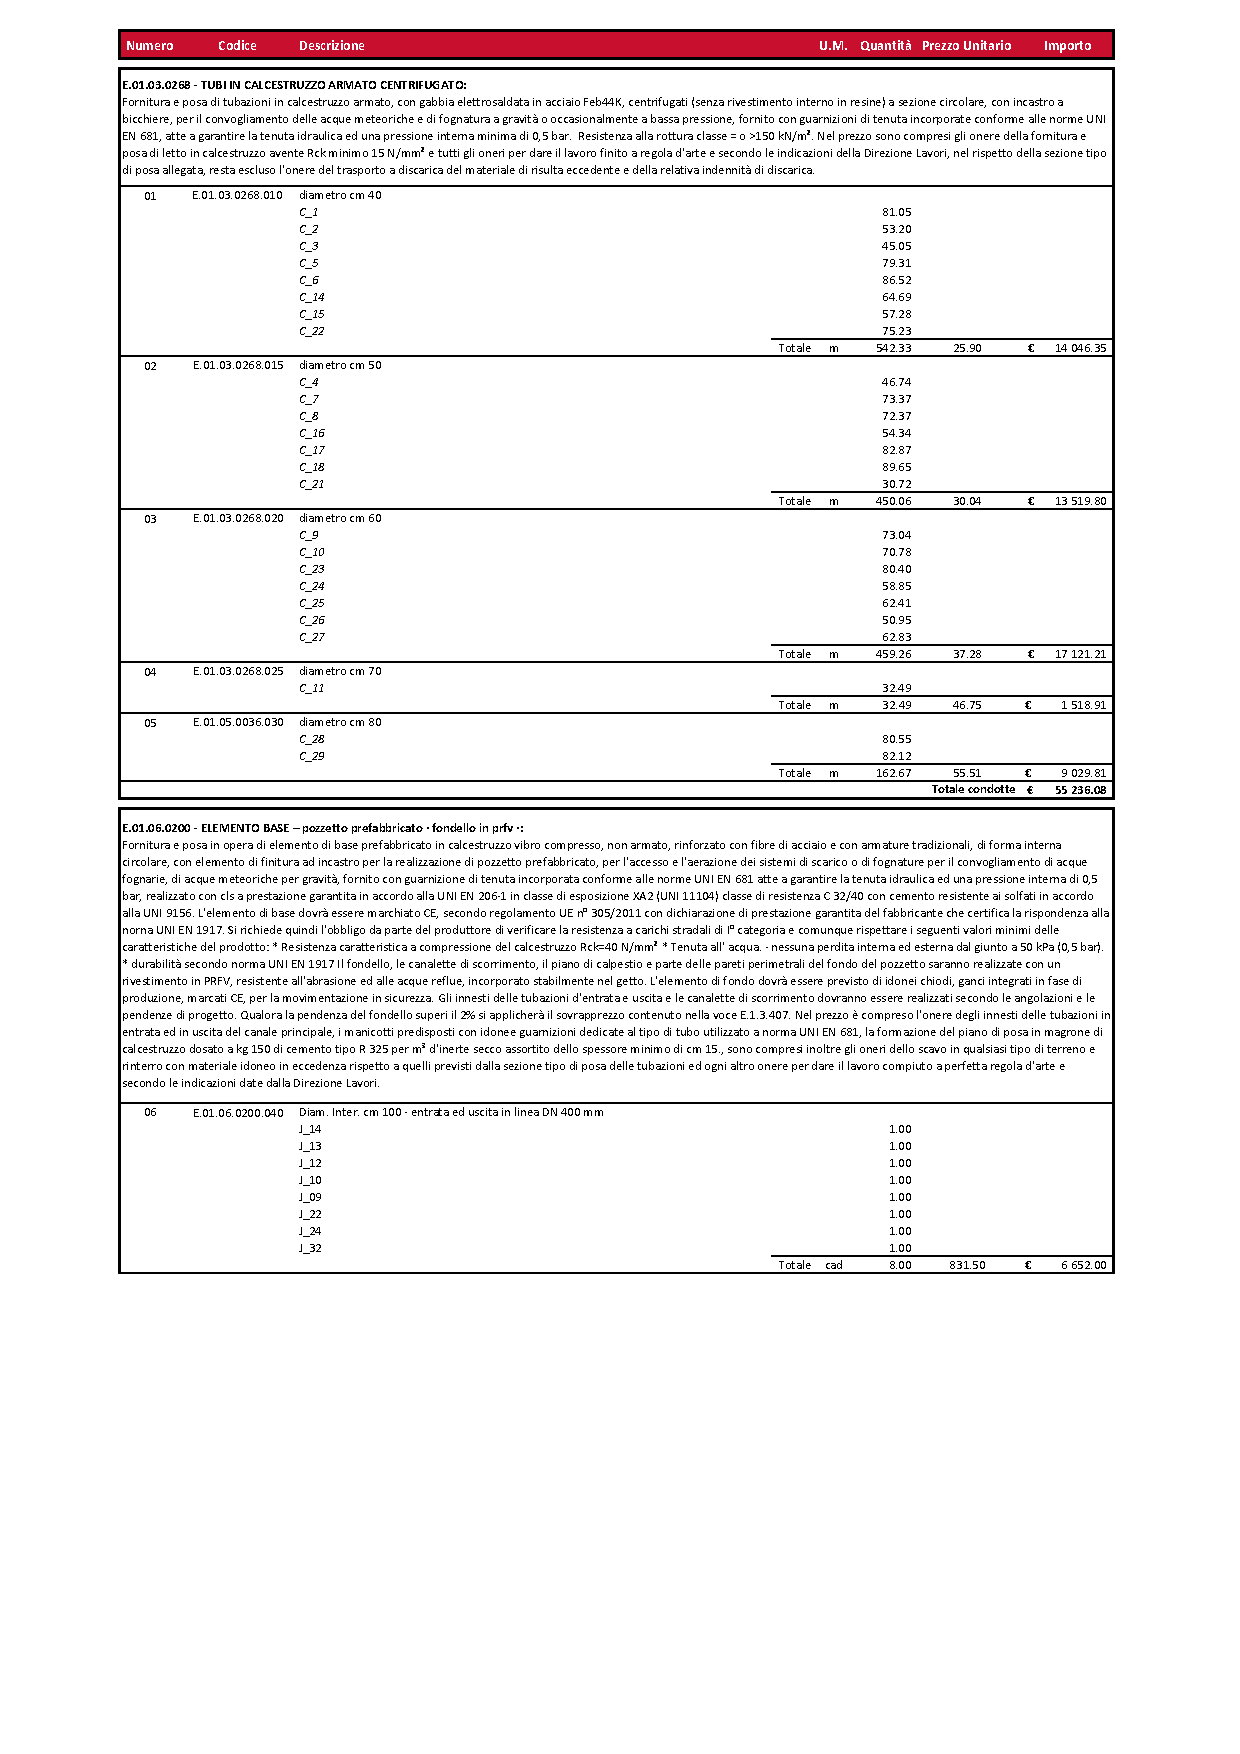
\includepdf[pages={1},pagecommand={\thispagestyle{plain},\section{Computo metrico estimativo}},addtotoc={1,section,1,Computo Metrico Estimativo,appendix:computo},offset=0 -5cm]{img/computo1.pdf}
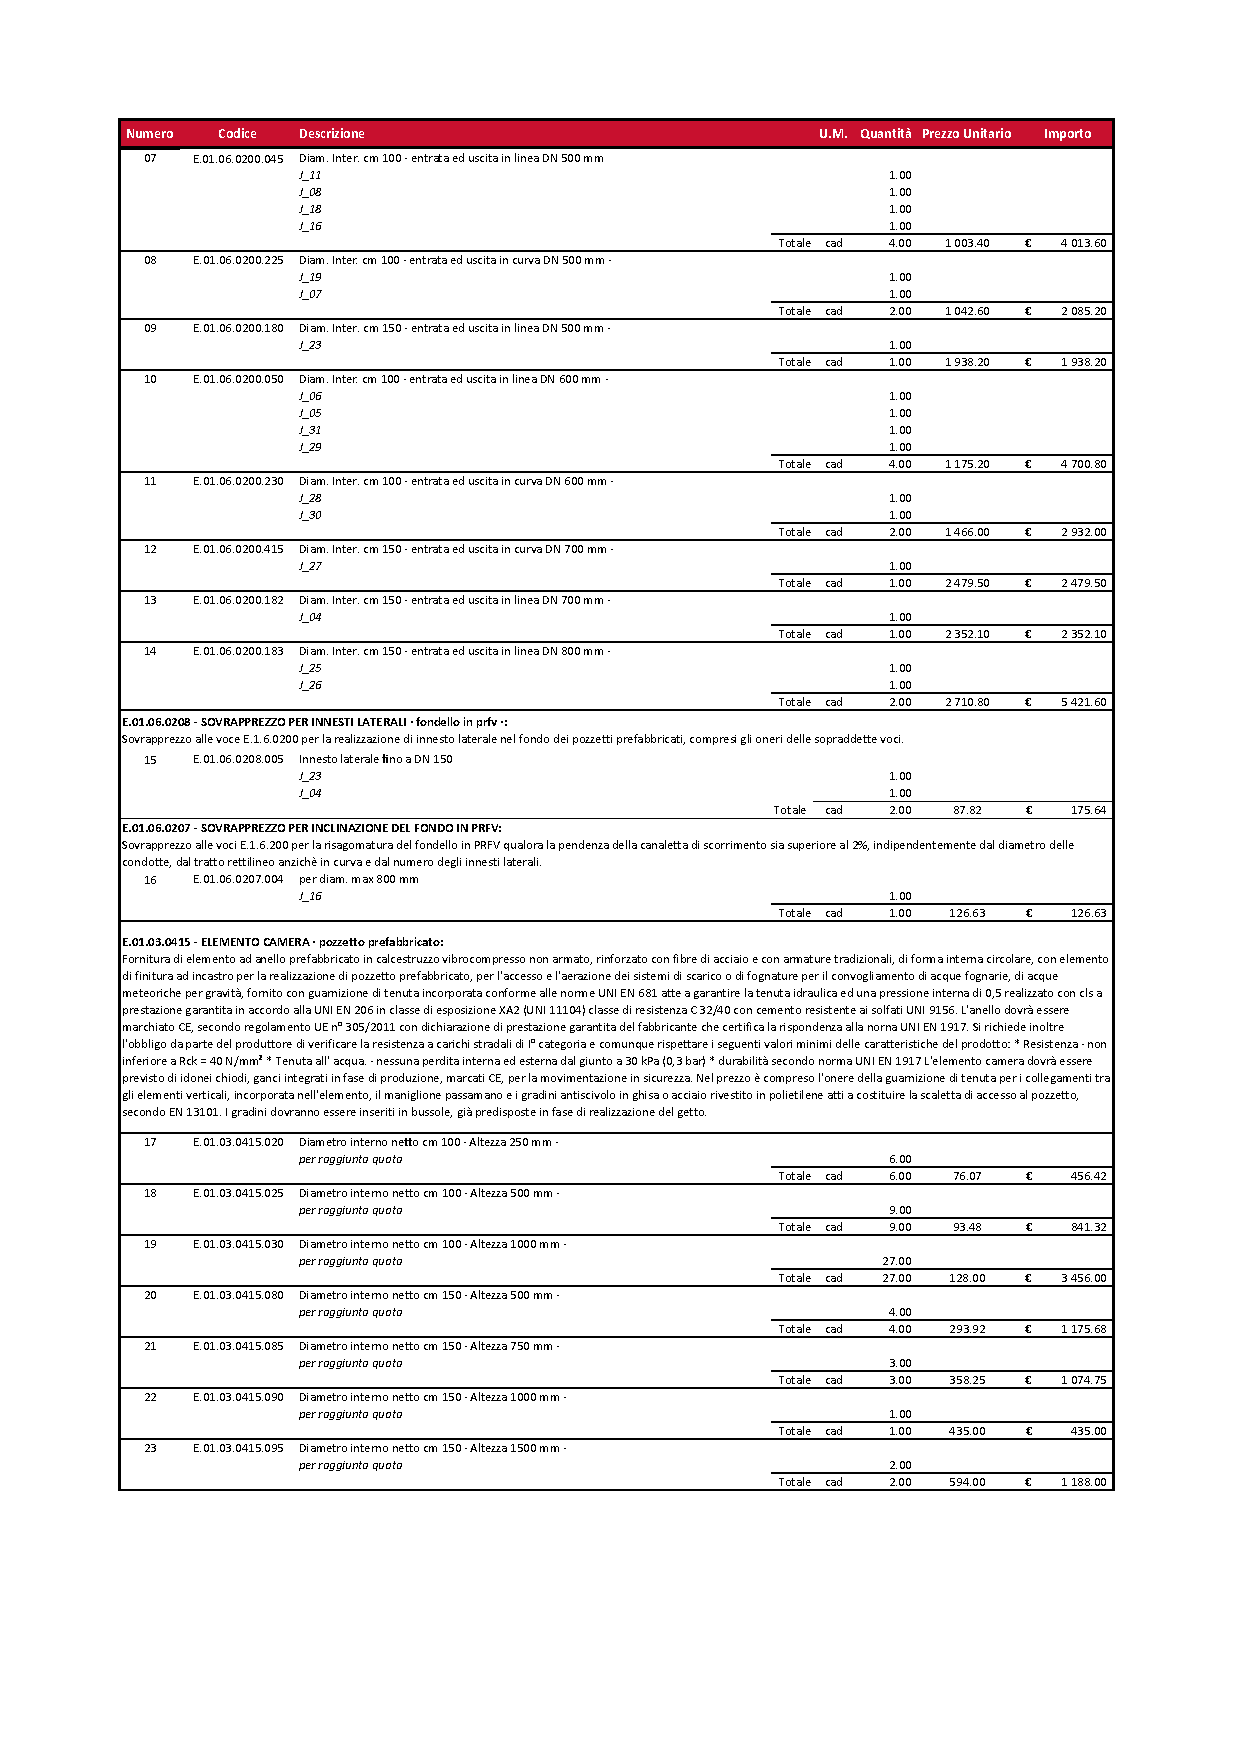
\includepdf[pages={1,2},pagecommand={\thispagestyle{plain}}]{img/computo2.pdf}

